\documentclass[a4paper,12pt,openbib]{article}

\usepackage{titling}
\usepackage[margin=0.5in,headsep=0.25in,footskip=0.25in]{geometry}
\usepackage{graphicx}
\usepackage{float}


\newcommand{\subtitle}[1]{
	\posttitle{
		\par\end{center}
		\begin{center}\large#1\end{center}
		\vskip0.5em
	}
}

\newcommand{\datacube}[3]{
\begin{figure}[ht!]
	\centering
	\setlength{\unitlength}{1cm}
	\begin{picture}(10,5)
		\put(0,0){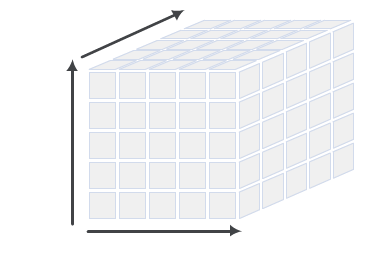
\includegraphics[height=5cm]{cube}}
		\put(1,4.5){#1}
		\put(-0.25,2){#2}
		\put(2,0.0){#3}
	\end{picture}
\end{figure}
}

\newcommand{\drilldown}[1]{
\begin{figure}[ht!]
	\centering
	\setlength{\unitlength}{1cm}
	\begin{picture}(1,1)
		\put(-2,0){
\includegraphics[height=1cm]{drill}}
		\put(-3.5,0.5){#1}
	\end{picture}
\end{figure}
}

\begin{document}

% title page
% TODO: Spruce it up
\title{CITS3401 Data Exploration and Mining\\
Project 1}
\subtitle{Medicare Australia Data Warehouse}
\author{Mitchell Pomery\\
21130887}
\maketitle
\abstract{
This document outlines the design choices for a data cube created to assist Medicare, an Australian Health-care Supporter, in providing the best service possible.
The original requirements were incomplete and so assumptions were made where necessary.
}
\clearpage

% document

\section*{Introduction}
\paragraph{}
Medicare Australia wishes to use data from it's previous years to assist in making decisions to improve their services, analyze expenditure and detect individuals who are abusing their system.
Each center stores information about visits in an Online Transaction Processing (OLTP) database, these are then collated at a state and country wide level.
The patient, doctor, treatment and prescriptions for each visit are stored.
This document outlines the data cube designed facilitate in the decision making processes of Medicare.

\section*{Requirements}
\paragraph{}
% TODO: List Requirements
The authors' interpretation of the requirements are listed below.

\begin{table}[h]
\centering
\begin{tabular}{|l|l|l|}
	\hline
		\textbf{Object} & \textbf{Restrictions} \\
	\hline
		Location & State or Territory in Australia \\
	\hline
		Center & 3 Centers in each State/Territory \\
	\hline
		Patient &  \\
	\hline
		Tests & Only one test will occur per visit. \\
	\hline
		Diseases & Only one disease will be diagnosed per visit maximum. \\
	\hline
		Referrals & Occur when a disease has been diagnosed. \\
	\hline
		Date & 2006 to 2011, broken down into quarters. \\
	\hline
\end{tabular}
\caption{Requirements}
\label{tab:requirements}
\end{table}

\subsection*{Assumptions}
\paragraph{}
Assumptions were made where the requirements were incomplete or insufficient, to simplify the schema and keep it manageable, and to make the scenario as realistic as possible.
% TODO: Assumptions
\begin{enumerate}
	\item Only a small number of patients, diseases, physicians, hospitals, specialists and pathology clinics exist.
	\item Doctors are irrelevant, only the name of the clinic matters.
	\item Patients will always visit a General Physician before seeing a specialist.
	\item The cost of treatment, as well as the person or company who pays for the treatment is irrelevant.
	\item People only visit medical centers in their own state.
	\item All data is complete and easily available in the desired format.
\end{enumerate}

\section*{Warehouse Schema}
\paragraph{}
A star schema was designed to make the data cube simpler, and the queries faster than a snowflake schema or fact constellation.
The date of the visit was broken into two dimensions, Year and Quarter, to allow for comparison between different years.
This allows us to see which diseases reoccur at high rates each year, and when they occur.
\paragraph{}
The requirements also state that Medicare is interested in using this data for analyzing several areas of their business.
They would like to be able to determine which patients frequently return for diagnosis and prescriptions and which doctors frequently refer patients to the same specialists.
The discovery of trends in diseases and referrals, and the discovery of outliers in patients, medical centers and treatment times would be beneficial for Medicare.

\begin{figure}[ht!]
	\centering
	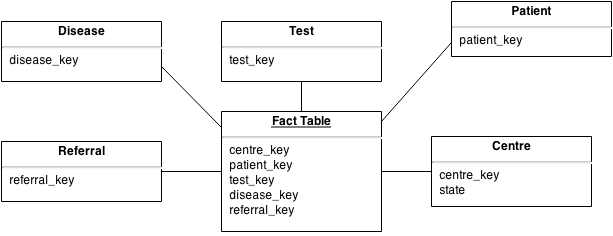
\includegraphics[width=15cm]{schema}
	\caption{Fact Table in Star Schema}
	\label{fig:schema}
\end{figure}

\section*{Prototype Warehouse}
\subsection*{Data Generation}
\paragraph{}
	Prototype data was generated using the Python script \texttt{gendata.py}.
	It takes sets of words for diseases, clinics, names, medical tests and states, creates random people and outputs information about their visits from 2006 to 2011.
	An attempt has been made to make it reflect reality, by restricting the average persons visits to a couple of times a year, charging based on the location visited and making a small percentage of users abuse the system each year.

\section*{Data Analysis}
\paragraph{}
	\texttt{Palo.xlsx} was created to import the data into the OLAP database for analysis, however due to issues with PALO, it was soon discarded.
	\texttt{search.py} was written to do data analysis on the data generated by \texttt{gendata.py}, and the output was manually entered into \texttt{Python.xlsx} .
	\texttt{search.py} enumerates all the possible elements for each dimension into several arrays, then counts the number of transactions that satisfy certain conditions, such as state, and places it into a table.
\paragraph{}
	Medicare Australia is then able to view the output data and determine what action, if any, needs to occur.
	By looking at the visits per patient per year, Medicare will be able to determine if any individuals are using their services abnormally, they will then be able to investigate if the visits are legitimate.
	By looking at the yearly breakdown of clinics, it is possible to see trends in patient numbers for each year.
	This is useful as it will allow Medicare to determine what areas are in need of upgraded infrastructure.

\section*{Scenarios}
\subsection*{Data Generation}

\clearpage
\section*{Data Cube}
\paragraph{}
	A visualization of the data cube is provided below:
\datacube{Tests}{Time}{Location}
\drilldown{}
\datacube{Tests}{Year}{State}
\drilldown{Drill Down On Year}
\datacube{Tests}{Quarter}{State}
\drilldown{Drill Down On State}
\datacube{Tests}{Quarter}{Clinic}
\drilldown{Drill Down On Tests}
\datacube{Diseases}{Quarter}{Clinic}
\drilldown{Drill Down On Diseases}
\datacube{Specialist}{Quarter}{Clinic}

\clearpage
\section*{Example Output}
\paragraph{}
	A visualization of the data cube is provided below:

\begin{figure}[ht!]
	\centering
	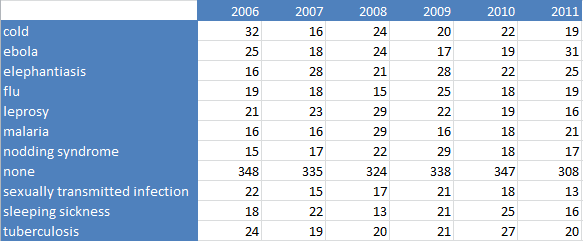
\includegraphics[width=15cm]{numberofdiseased}
	\caption{Number of patients diagnosed with a disease}
	\label{fig:disease}
\end{figure}

\begin{figure}[ht!]
	\centering
	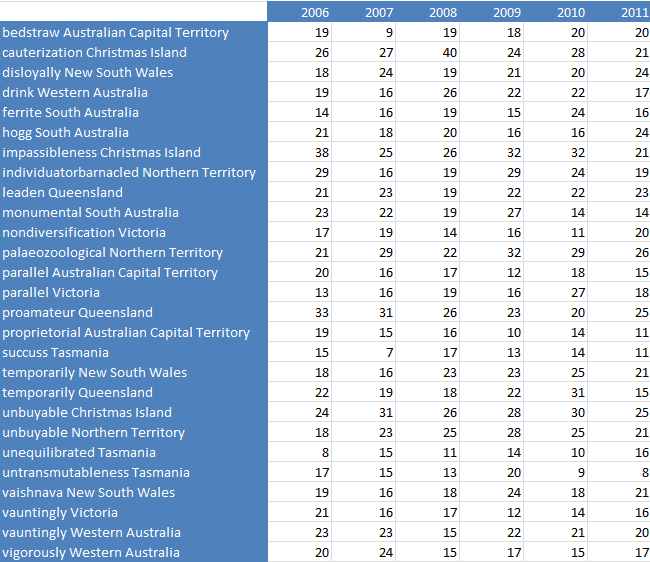
\includegraphics[width=15cm]{visitsperclinic}
	\caption{Number of visitors to each clinic}
	\label{fig:{visitsperclinic}}
\end{figure}

\begin{figure}[ht!]
	\centering
	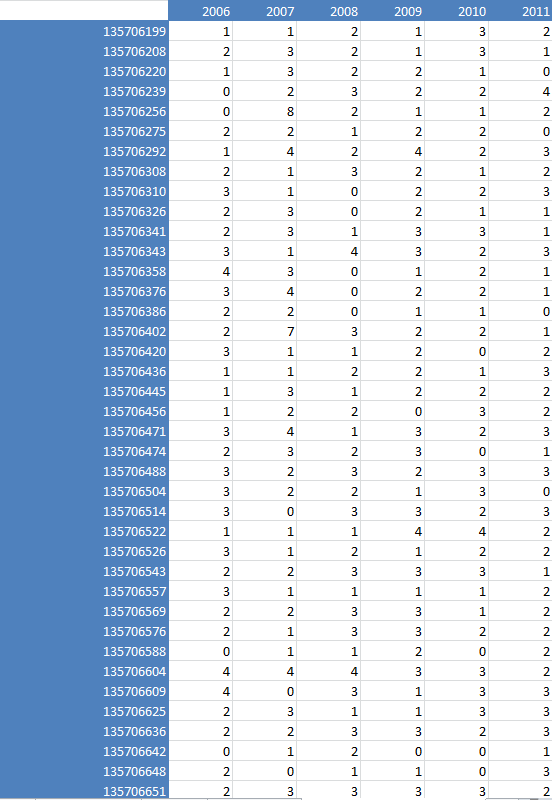
\includegraphics[width=15cm]{visitsperperson}
	\caption{Number of visits by an individual}
	\label{fig:visitsperperson}
\end{figure}

\end{document}